\section{Learning Dynamics of Occupancy Grid}
\label{sec:learning_dynamics_of_env}

\subsection{Previous Work}
Learning the dynamics of an environment is a subject with ongoing research.
An early system for mapping the dynamics of the environment in a occupancy grid was the Temporal Occupancy Grid (TOG) proposed by Arbucle et al. \cite{Arbuckle2002}. The TOG system maintains several occupancy grids spanning different time periods. This requires storing the observations for the longest period. It can be difficult to determine the periods needed to estimate the different and changing dynamic behaviors in the environment.

Biber and Duckett \cite{Biber2005} proposes a method for mapping environment dynamics with maps that represent observations taken over different periods of time. The method is here denoted as Temporal Sample Map (TSM). The maps are updated by incorporating measurements using different recency weighted running average functions. These functions are estimated by removing random observations. The highly dynamic obstacles are considered as outliers and up to $50\%$ of them are removed by using the median measurement.

An avenue of thought that has received quite a lot of attention is  representing dynamic environments by Markov processes.  
A Markov grid was introduced by Sarinnen et al. \cite{Saarinen2012} called Independent Markov Chain grid map (IMAC). This method represents each cell as the Markov process in figure \ref{fig:markow_occupancy_model} which can be in either of the states; free or occupied. 

\begin{figure}[tbph]
	\centering
	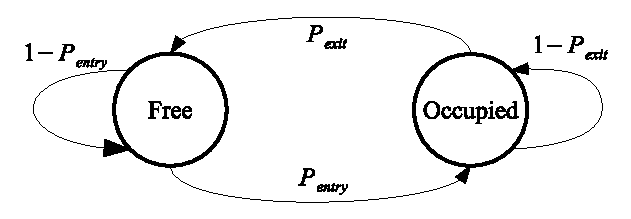
\includegraphics[width=0.7\linewidth]{chapters/mapping_of_dynamic_areas/figures/markow_occupancy_model}
	\caption{Markow chain for occupancy states borrowed from \cite{Saarinen2012}}
	\label{fig:markow_occupancy_model}
\end{figure}

\todo{DRAW NEW FIGURE -> STATE TRANSISITON}

Transitions between states are modeled as two Poisson processes. The transition probabilities $P_{exit}$ and $P_{entry}$ is estimated as Gamma distributions with rate parameters $\hat{\lambda}_{exit}$ and $\hat{\lambda}_{entry}$.
The parameters are given by the number of state changes divided by the number possible state changes as shown in equation \ref{eq:imac_learning}.

\begin{align}
	P_{exit} \sim \hat{\lambda}_{exit} &= \frac{\#events:\; occupied\; to\; free + 1}{\#observations\; when\; occupied + 1} \label{eq:imac_learning}\\
	P_{entry} \sim\hat{\lambda}_{entry} &= \frac{\#events:\; free\; to\; occupied + 1}{\#observations\; when\; free + 1}
	\nonumber
\end{align}


Meyer-Delius et al. \cite{Meyer-Delius2012} proposes to model the Markov process using a Hidden Markov Model (HMM) where the states are not directly observable.
This allows for  including observation uncertainty in the learning method.
The Markov parameters can be learned either offline or online.
The offline approach requires storing all observations and then learn the parameters using an expectation-maximization algorithm. 
The requirement of storing observations makes the offline version unsuitable for life-long mapping. 
An online parameter learning algorithm was developed by Mongillo and Deneve \cite{Mongillo2008}. 
It eliminates the need for storing the whole observation set. 
Instead only 16 values are needed to continuously learn the parameters for each cell. 
has to be stored for each cell and the iterative learning can be done online. 
The online method is capable of handling changing dynamics by using a forget factor. 

A different approach to mapping the dynamics is the Frequency Map Enhancement (FreMEn) proposed by Krajník et al. \cite{Krajnik2014}. This method models the dynamics of each cell by its primary frequency components.
The method investigated further in section \ref{sec:fremen}.

Table \ref{tab:learners_characteristics} shows characteristics of the discussed methods for learning dynamics. 

\begin{table}[htbp]
    \centering
    \caption{Characteristics of methods to learn dynamics in occupancy grids.}
    \label{tab:learners_characteristics}
    \begin{tabular}{p{2.6cm} | p{1.6cm} | p{4.cm} | p{2.6cm}}
        \toprule
        \textbf{Name} & \textbf{Memory} & \textbf{Dynamic representation} & \textbf{Learning method}  \\
        \rowcolor[gray]{0.925}
        TOG & High & OG for multiple time scales & Online batch  \\
        TSM & Medium & OG for multiple time scales & Random sample replacement  \\
        \rowcolor[gray]{0.925}
        IMAC & Low & Markov parameters & Online iterative  \\
        HMM - Offline & High & Markov parameters & Offline batch  \\
        \rowcolor[gray]{0.925} 
        HMM - Online & Low & Markov parameters & Online iterative  \\
        FreMEn & Low & Frequency components & Online iterative \\
        \bottomrule
    \end{tabular}
\end{table}

\subsection{Methods Ability to Learn Markov Processes}
The described  methods that models dynamics with Markov processes are compared with a simple 1D simulation where a grid cell is occupied by a dynamic obstacle. 
Whether the cell is occupied or free is controlled by a Markov process with $P_{entry}=0.9$ and $P_{exit}=0.2$. 
The process is observed by a one dimensional range sensor with zero mean Gaussian noise with a standard deviation of $0.5cell$.
Thus the probability of measuring too short is $0.16$, in which case the online-HMM are propagated one step without adding new information and the IMAC is left unchanged.
There is an equal probability for the sensor measuring a range too far, which results in a reading of an empty cell independently of the cell's state. 
Figure \ref{fig:markow_learning} shows that IMAC is unable to converge to the correct transition probabilities, whereas the HMM-online method that incorporate the uncertainties in measurements slowly converges toward them.

Considering that the dynamic learner receives observations from the static mapper, each observation would be a complete static mapping cycle. With a cycle at one minute it will take $33.3$ hours to learn the Markov parameters. 

\begin{figure}[htbp]
    \centering
    \begin{subfigure}[t]{0.45\textwidth}
        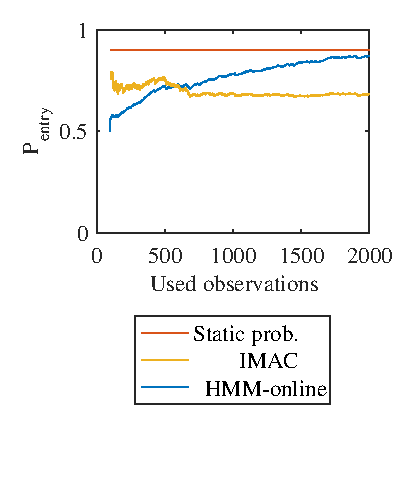
\includegraphics[width=1.0\textwidth]{chapters/mapping_of_dynamic_areas/figures/markow_learn_1d_entry}	
        %\caption{}
        %\label{fig:markow_learn_1d_entry}
    \end{subfigure}
    \begin{subfigure}[t]{0.45\textwidth}
        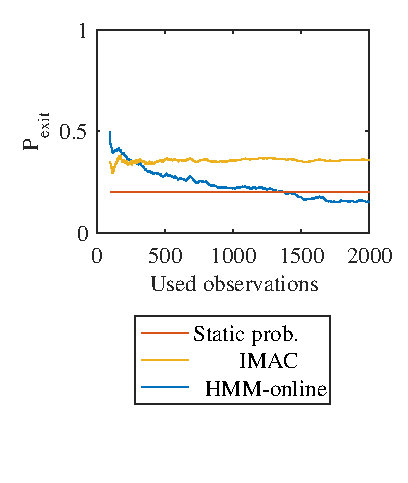
\includegraphics[width=1.0\textwidth]{chapters/mapping_of_dynamic_areas/figures/markow_learn_1d_exit}
        %\caption{}
        %\label{fig:markow_learn_1d_exit}
    \end{subfigure}
    \caption{Learned state transition probabilities compared to the simulated Markow process.}
    \label{fig:markow_learning}
\end{figure}
